\documentclass[a4paper,12pt]{article}
\usepackage[brazil,english]{babel}
\usepackage[utf8]{inputenc}
\usepackage[T1]{fontenc}
\usepackage{indentfirst}
\usepackage[pdftex]{graphicx}
\usepackage{subcaption}
\usepackage{geometry}
\usepackage{color}
\usepackage{float}
\geometry{a4paper, margin=2cm}

\title{Ajuste de Equação de Volume Comercial para a Espécie Goupia Glabra (Cupiúba) utilizando o Modelo de Husch: Um Estudo de caso aplicado à Concessão Florestal de Altamira-PA} %% Titulo do Artigo

\author{Jessica Teixeira Araujo \\ Prof. Dr. rer. nat. João Marcelo Brazão Protázio}

\date{\today} %% Autor do Projeto

\begin{document}
	
\maketitle

\selectlanguage{english}
\begin{abstract}
\noindent
The work aims to develop a commercial volume equation for the species Hymenolobium elatum (Angelim-Pedra) with rigorous cubing based on the measurement of logs from the Forest Concession of the National Forest of Altamira-PA, the model of simple entry known in the forest sciences was selected as Husch's model for its easy and simple application, seeking to offer environmental agencies, companies and forest sector producers practicality and greater volumetric precision in forest management plans.
\end{abstract} %% Abstract

\selectlanguage{brazil}
\begin{abstract}
\noindent
O trabalho visa desenvolver equação de volume comercial para a espécie Hymenolobium elatum (Angelim-Pedra) a partir da cubagem rigorosa baseada em dados obtidos da concessão florestal da Floresta Nacional de Altamira-PA. Para isso foi selecionado o modelo conhecido nas ciências florestais como Modelo de Husch e sua versão linearizada, pela sua fácil aplicação, buscando assim oferecer aos órgãos ambientais, empresas e produtores do setor florestal praticidade e maior precisão volumétrica nos planos de manejo florestal.
\end{abstract} %% Resumo

\section{Introdução}

Os métodos usuais de estimativa de volume comercial de árvores na atividade de manejo florestal utilizam o Fator de Forma (FF) no valor de 0.7, que estabelece a relação entre o volume de madeira e o volume do cilindro, utilizando-se a área transversal da árvore à altura do peito e a altura do fuste comercial. A outra forma é a equação de volume geral para todas as espécies, geralmente de dupla entrada, com a variável volume sendo a dependente em função de duas variáveis independentes: o diâmetro a altura do peito (DAP) e a altura comercial. As duas formas de cálculo de estimativas de volume são norteadas pela Instrução Normativa de 10 de setembro de 2015 para o estado do Pará, Secretária de Estado e Meio Ambiente e Sustentabilidade (SEMAS), onde se estabelece que no primeiro Plano Operacional Anual (POA) pode ser usado o FF = 0.7 e que se desenvolva uma equação de volume nos próximos POA´s do Plano de Manejo Florestal Sustentável (PMFS), assim como a Resolução N° 406, de 02 de fevereiro de 2009 do Conselho Nacional de Meio Ambiente – CONAMA.

A problemática envolvida na precisão dos dois métodos são duas: a estimativa da altura em florestas nativas, onde muitas vezes a falta de visibilidade e a inexperiência do mensurador, entre outros fatores, interferem substancialmente nos resultados (Moura, 1994), bem como o uso de FF único ou apenas uma Equação Geral para toda população florestal, as espécies apresentam em seus troncos formas distintas, gerando estimativas imprecisas em algumas espécies como no caso do Cupiúba, engenheiros florestais com experiência em manejo florestal na região amazônica tem ciência que a espécie apresenta forma de tronco mais cilíndrica que outras espécies. Baseado nessas informações foi selecionado o modelo de simples entrada de Husch para o ajuste da equação de volume comercial da espécie Cupiúba.

Em se tratando de equações volumétricas, as variáveis dendrométricas necessárias para a determinação do melhor modelo são: DAP, Altura comercial e volume comercial, porém como já foi descrito na introdução a variável altura é de difícil acesso e precisão não será utilizada no presente trabalho. 

Os dados de cubagem serão oriundos dos romaneios, cadeia de custódia da madeira explorada e comercializada, mais os dados de inventário florestal pré-exploratório, gerados pela atividade manejo florestal sustentável em áreas de concessões florestais estaduais e federais.

Os dados de cadeia de custódia são uniformes para todas as empresas, gerando milhares e com o passar dos anos milhões de dados de volume real de árvores exploradas e comercializadas. A palavra comercializada garante que o volume comercial é real, pois foi romaneada na floresta e depois conferida por quem comprou na serraria. Baseado também nessa cadeia de custódia que é pago o metro cúbico (m³) da madeira produzida para o estado ou federação periodicamente pelas empresas ao SFB.

Além da cadeia de custódia, com o número da tora, é informado aos órgãos ambientais e gestores também o número da árvore, onde o somatório do volume das toras equivale ao volume comercial por árvore e o somatório dos comprimentos das toras equivale a altura comercial.  Os dados de diâmetro à altura do peito para o ajuste da equação serão obtidos do inventário florestal pré-exploratório (censo).

\section{Materiais e Métodos}

\subsection{Conjunto de Dados}
Para realização do estudo foram obtidos  dados gerados pelas empresas concessionárias, com contrato ativo junto ao Serviço Florestal Brasileiro (SFB) que por sua vez gerenciam seus respectivos contratos de concessão florestais e cedeu as informações. Os dados tem origem na Floresta Nacional de Altamira, no estado do Pará.

Foi selecionada a espécie Cupiúba, pois as estimativas volumétricas baseadas no Fator de Forma 0.7 subestimam o volume, pois seu fuste tende a ser cilindríco, faltando assim crédito virtual de madeira nas operações comerciais dos Planos de Manejo Florestal Sustentável na Amazônia principalmente no primeiro POA, além da espécie possuir alta relevância econômica.

O total de árvores cubadas é 205, sendo que aproximadamente 70\%=144 dos indivíduos serão utilizados no ajuste do modelo volumétrico e as demais proximadamente 30\%=61 árvores serão utilizadas para a validação do modelo.

\begin{figure}[H]
\centering
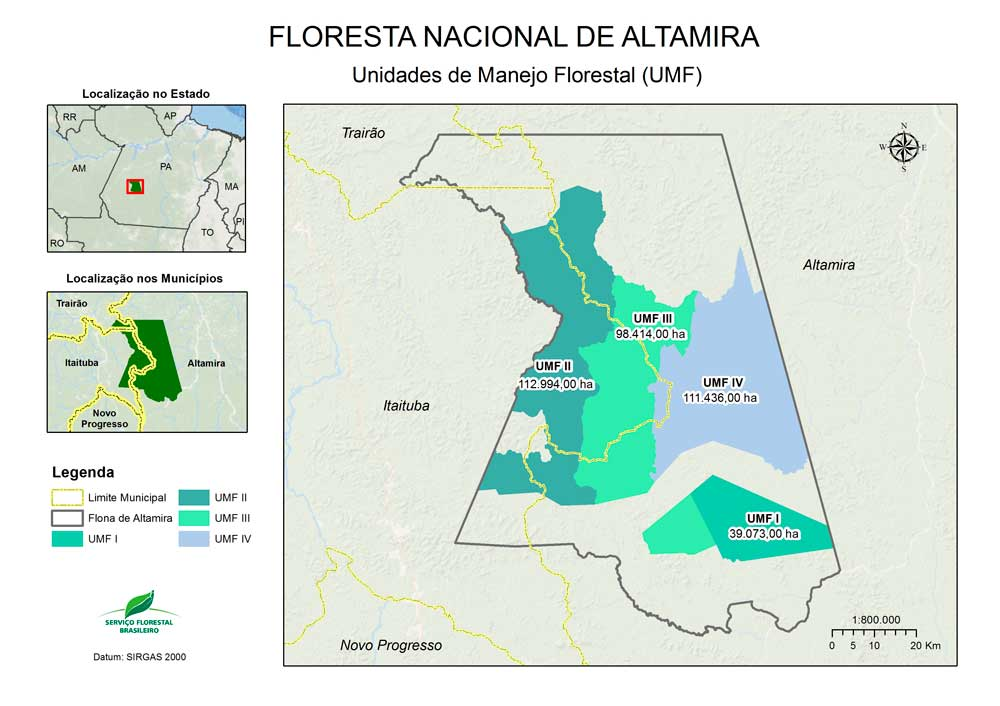
\includegraphics[width=0.9\textwidth]{flora.jpg}
\caption{Localização da Floresta Nacional de Altamira e suas Unidades de Manejo florestal.}
\label{mapa}
\end{figure}

\subsection{Modelo volumétrico de Husch}

O modelo selecionado foi o de Husch, baseado na praticidade de sua aplicação, facilmente ajustado em programas populares como o Excel e definido como:

\begin{center}
	\begin{equation}\label{m1}
	v = a d^{b}
	\end{equation}
\end{center}
onde $v$ e $d$ são respectivamente o volume comercial da árvore ($m^3$) o o diâmetro à altura do peito ($m$) e $a$ e $b$ são parâmetros espécie-específicos. 

Por outro lado, a versão linearizada do modelo de Husch é dada por:

\begin{center}
	\begin{equation}\label{m2}
	\hat{v} = \hat{a} + b \hat{d}
	\end{equation}
\end{center}

onde $\hat{v}=\ln v$ e $\hat{d}=\ln d$ são respectivamente o volume comercial o diâmetro à altura do peito das árvores e $\hat{a}=\ln a$ e $b$ são parâmetros espécie-específicos. 

\section{Resultados e Discussão}

\subsection{Estatística Descritiva Básica}

Logo abaixo, na Tabela \ref{t1} apresentamos a estatística descritiva básica das variáveis originais $v$ e $d$ apresentados no experimento.

\begin{table}[h]
\centering 
\caption{Estatística descritiva básica do diametro e do volume original.} 
\label{t1}
\begin{tabular}{llllll}
\hline
variável & min & max & média & dp & cv \\
\hline
$v$ & 1.511 & 13.566 & 4.886  & 2.241 & 0.458  \\
$d$ & 0.500  & 1.305 & 0.766 & 0.150 & 0.197  \\
\hline
\end{tabular}
\end{table}

\subsection{Ajuste do Modelo}

Os resultados relativos ao ajuste do modelo de Husch e à sua versão linearizada, são apresentados na Tabela \ref{t2}. A partir dos resultados apresentados, podemos dizer que o modelo mais adequado para a obtenção da estima o volume de madeira comercial da espécie Cupiúba neste área de estudo é o modelo de Husch linearizado. Podemos ver isto também visualmente na Figura \ref{f1}.

\begin{figure}[H]
\centering
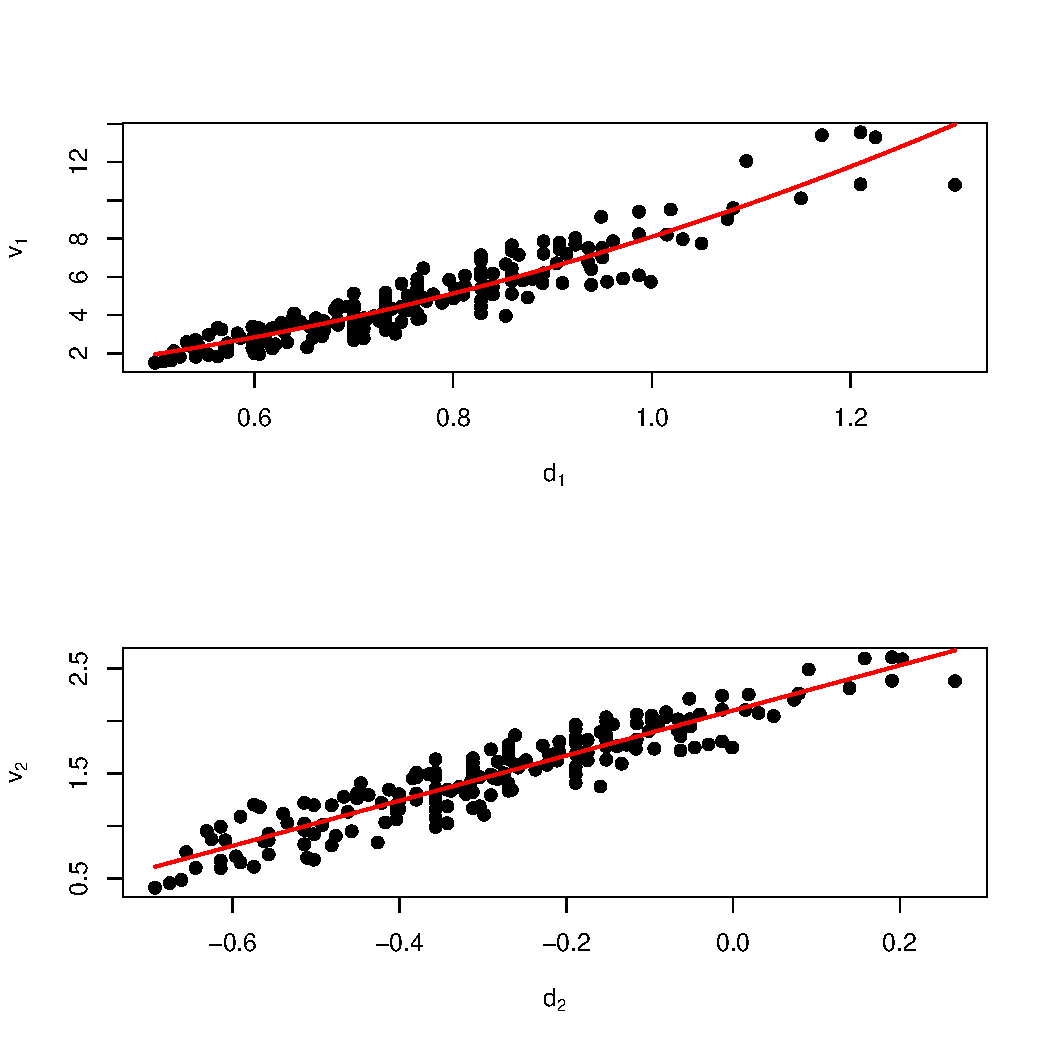
\includegraphics[width=0.9\textwidth]{result.pdf}
\caption{Localização da Floresta Nacional de Altamira e suas Unidades de Manejo florestal.}
\label{f1}
\end{figure}

\begin{table}[h]
\centering 
\caption{Resultado do Ajuste ao Modelo Husch e à sua versão linearizada.} 
\label{t2}
\begin{tabular}{lllll}
\hline
Modelo & $a$ & $b$ & erro (\%)  & AIC \\
\hline
Husch & 10.34 & 1.90 & 1.43 &  10000\\
Husch Linearizado & 2.42 & 2.23 & $4.23 \times 10^{-13}$ & -4800 \\
\hline
\end{tabular}
\end{table}

A partir dos resultados apresentados na Tabela \ref{t2}, podemos dizer que o modelo mais adequado para a estimar o volume de madeira comercial da espécie Cupiúba neste área de estudo é o modelo de Husch linearizado.

\section{Bibliografia Utilizada}

CONAMA. Conselho Nacional do Meio Ambiente. Resolução n° 406, de 02 de fevereiro de 2009. Estabelece parâmetros técnicos a serem adotados na elaboração, apresentação, avaliação técnica e execução de Plano de Manejo Florestal Sustentável-PMFS com fins madeireiros, para florestas nativas e suas formas de sucessão no bioma Amazônia. Diário Oficial da União: secao 1, Brasilia-DF, ano 147, nº 26, de 06/02/2009. Brasília, DF. Pág. 100.

MOURA, J. B. Estudo da forma do fuste e comparação de métodos de estimativa volumétrica de espécies florestais da Amazônia brasileira. 1994. 113 f. Dissertação (Mestrado em Ciências Florestais) – Universidade Federal de Curitiba, Curitiba.

SEMAS-PA. Secretaria de Meio Ambiente e Sustentabilidade do Pará.  Instrução Normativa de 10 de setembro de 2015. Dispõe sobre procedimentos técnicos para elaboração, apresentação, execução e avaliação técnica de Plano de Manejo Florestal Sustentável – PMFS nas florestas nativas exploradas ou não e suas formas de sucessão no Estado do Pará, e dá outras providências. Diário Oficial do Estado do Pará, n. 32969 de 11/09/2015. Belém, PA. Páginas de 37-57.

R Core Team (2013). R: A Language and Environment for Statistical Computing. R Foundation for Statistical Computing, Vienna, Austria. URL http://www.R-project.org/.

SFB. Serviço Florestal Brasileiro. Seis florestas nacionais abrigam concessão florestal. 2016. Disponível em: http://www.florestal.gov.br/florestas-sob-concessao. Acesso em :28 jan. 2021.

\end{document}